% mycsrf 'for beeing included' snippet template
%
% (c) Karsten Reincke, Frankfurt a.M. 2012, ff.
%
% This text is licensed under the Creative Commons Attribution 3.0 Germany
% License (http://creativecommons.org/licenses/by/3.0/de/): Feel free to share
% (to copy, distribute and transmit) or to remix (to adapt) it, if you respect
% how you must attribute the work in the manner specified by the author(s):
% \newline
% In an internet based reuse please link the reused parts to mycsrf.fodina.de
% and mention the original author Karsten Reincke in a suitable manner. In a
% paper-like reuse please insert a short hint to mycsrf.fodina.de and to the
% original author, Karsten Reincke, into your preface. For normal quotations
% please use the scientific standard to cite
%


%% use all entries of the bibliography

\subsection{Laborejo ($\bigstar$ $\bigstar$ $\bigstar$)}

\parpic(2cm,2cm)[r][t]{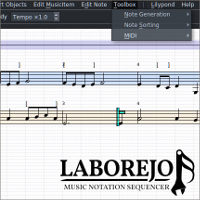
\includegraphics[width=1.8cm]{logos/laborejo-300dpi.png}}
\label{Laborejo}\acc{Laborejo} ist Teil einer Software Suite und sieht sich
selbst als \enquote{MIDI sequencer based on classical music notation}. Es ziele
hauptsächlich darauf, traditionelle Musik zu komponieren und zu produzieren.
Anders als andere Notationssysteme sei \acc{Laborejo} aber nicht dazu gedacht,
Notenblätter zu erzeugen, sondern auf und mit dem Rechner zu musizieren.\footcite[vgl.][\nopage wp.]{Hilbricht2019a} Eine spezielle Download-Page bietet entsprechende Pakete für die einzelnen Distributionen\footcite[vgl.][\nopage wp.]{Hilbricht2019b}, die Installation ist aber nicht trivial, weil man u.a. auch das \acc{Jack Audio Connection Kit} installiert und gestartet haben muss. Für \acc{laborejo} selbst gibt es eine ausführlich deutsch-sprachige Dokumentation.\footcite[vgl.][\nopage wp.]{Hilbricht2019c}

Um die Quellen einzusehen, muss man die kleine Klippe umschiffen, das Repository nicht unter GitHub zu suchen. Vielmehr bietet der Autor ein gesondert gehostetes GIT-Repository an.\footcite[vgl.][\nopage wp.]{Hilbricht2021a} Das Repository enthält die GPL-3.0 unter dem Dateinamen \texttt{LICENSE}. \acc{Laborejo} ist also freie Software.

Ausgehend von der Selbsteinschätzung, dass \enquote{unlike other notation editors Laborejo is not meant primarily to print out sheets of notation but to create music for your computer}\footcite[vgl.][\nopage wp.]{Hilbricht2019a}, dürfen wir sagen, dass dieses Programm als Frontend für unsere \LaTeX\ bezogenen Zwecke eher nicht in Frage kommt. Die Sorgfalt und Update-Frequenz der Softwareentwicklung zeigt aber, dass für das 'Sequencing' eine interessant Alternative ist.\footnote{Zwischen der Version 1.4 und aktuellen Version dieses Textes hat mich der Laborejo-Autor Nils Hilbricht dankenswerterweise über Neuentwicklungen informiert. Was noch bis 2019 galt, ist jetzt überholt. Die Links habe ich entsprechend geupdated. Besonders wertvoll war der Hinweis, dass die Version 0.8, die Ubuntu 20.04 beiliegt, mittlerweile einen völlig irrigen Eindruck vermittelt: Tatsächlich gibt es seit 2020 nämlich die Version 2.0.0} Das soll uns drei Sterne wert sein.
% this is only inserted to eject fault messages in texlipse
%\bibliography{../bib/literature}
